\documentclass{beamer}
%\mode<presentation>
\usepackage[utf8]{inputenc}
\usetheme{CambridgeUS}
\usecolortheme{albatross}
\usepackage{amsmath,amssymb,amsfonts}
\usepackage{mathpazo}
\usepackage{graphicx,tabularx,epsfig}
\title{Hidrodinamika}
\author{Bagoly Attila}
\date{2013.01.28}
\institute{ELTE}

\begin{document}

\begin{frame}
  \titlepage
\end{frame}



\section{Nemrelativisztikus hidrodinamika}

\subsection{Az egyenletek}
\begin{frame}
%\setbeamercovered{dynamic}
\frametitle{Bevezető}
\begin{itemize}
\item Alapvető keresett mennyiségek: $\vec{v}(\vec{r},t)$, $\rho(\vec{r},t)$, $p(\vec{r},t)$, $T(\vec{r},t)$
\item Ideális folyadék: összenyomhatatlan
\item Tökéletes folyadék: elhanyagolható a viszkozitás és a hővezetés
\item Állapotegyenlet: lokális termodinamikai egyensúlyt feltételezünk, kell egy nem "hidrodinamikai" egyenlet (pl. $\epsilon=\kappa p$), 
\end{itemize}
\end{frame}


\subsection{A hidrodinamika egyenletei}

\begin{frame}
\frametitle{Kontinuitási egyenlet}
\begin{center}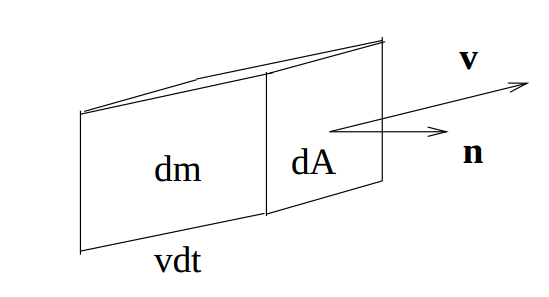
\includegraphics[width=0.40\textwidth]{pic/f1.png}\end{center}
Ábra alapján a felületen kiáramló tömeg: $dm=\rho \vec{v}\vec{n}dAdt$
Az anyag megmarad tehát ami a felületen kiáramlik "bentről" eltűnik, azaz: 
\begin{equation*}
\frac{d}{dt}\int \rho dV+\oint \rho \vec{v}d\vec{A}=0
\end{equation*}
Az felületi integrál Gauss tétel segítségével könnyedén átírható és így kapjuk a differenciális alakot: 
\begin{equation*}
\frac{\partial \rho}{\partial t}+\nabla \cdot (\rho \vec{v})=0
\end{equation*}
\end{frame}

\begin{frame}
\frametitle{Euler-egyenlet}
Hidrodinamikai derivált:
\begin{columns}
\column{0.70\textwidth}
	\begin{equation*}
		\Delta  \phi = \phi (\vec{r}+\Delta\vec{r}, t+\Delta t)-\phi (\vec{r},t) \Rightarrow 
	\end{equation*}
	\begin{equation*}
		\frac{d \phi}{dt}=\frac{\partial \phi}{\partial t}+(\vec{v}\nabla)\phi
	\end{equation*}
\column{0.30\textwidth}
	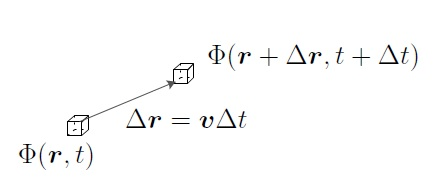
\includegraphics[width=1.00\textwidth]{pic/f2.jpg}
\end{columns}
Kontinuummechanika mozgásegyenlete: $\rho \frac{d \vec{v}}{dt}=\vec{f}+div(\sigma)$.
Tökéletes folyadékra érvényes (Pascal törvény): $\sigma=-pE$.
Ezek alapján felírhatjuk a tökéletes folyadékra érvényes mozgásegyenletet ($f=0$): 
\begin{equation*}
\frac{\partial \vec{v}}{\partial t}+(\vec{v}\nabla)\vec{v}=-\frac{\nabla p}{\rho}
\end{equation*}
\end{frame}

\begin{frame}
\frametitle{Euler-egyenlet kicsit másként}
Láttuk, hogy az anyag megmarad és a megmaradását a kontinuitás egyenlet írja le. Mi marad még meg? 

Ha nem lenne nyomás tag akkor az impulzussűrűség ($\rho \vec{v}$) megmaradna. Az impulzus meg nem maradást is felírhatjuk kontinuitás egyenlethez hasonlóan! Olyan kontinuitás egyenlet amelyben forrás tag jelenik meg! (Ezeket mérlegegyenleteknek nevezzük) 
Formálisan:
\begin{equation*}
\frac{\partial}{\partial t}\int \rho \vec{v} dV+\oint (\rho\vec{v})\circ\vec{v}d\vec{A}+\oint p d\vec{A}=0
\end{equation*}
A felületi integrálokat térfogativá alakítva kaphatjuk meg az egyenlet differenciális alakját:
\begin{equation*}
\frac{\partial\rho \vec{v}}{\partial t}+(\vec{v}\nabla)\rho\vec{v}=-\nabla p
\end{equation*}
Miért néztük meg ezt a konstrukciót? Még van "megmaradó" mennyiség!
\end{frame}

\begin{frame}
\frametitle{Energia egyenlet}
Az előbbihez hasonlóan az energiasűrűség meg nem maradására is mérlegegyenletet írhatunk fel. A "megmaradó" mennyiség most az energiasűrűség, melynek a forrástagja a nyomásból származó teljesítmény.
\begin{equation*}
\frac{\partial}{\partial t}\int \rho\epsilon dV+\oint \rho\epsilon\vec{v}d\vec{A}+\oint p\vec{v} d\vec{A}=0
\end{equation*}
Az integrálokat átalakítva kaphatjuk meg az energia egyenlet differenciális alakját:
\begin{equation*}
\frac{\partial\rho \epsilon}{\partial t}+\nabla\rho\epsilon\vec{v}=-\nabla p\vec{v}
\end{equation*}
\end{frame}

\begin{frame}
\frametitle{Összegzés}
\begin{itemize}
\item Tehát a 6 darab keresett mennyiségre megalkottuk a 6 darab egyenletet.
\item Ez egy 6 ismeretlenes parciális differenciálegyenlet rendszer, nem lineáris!
\item Kezdő és peremfeltételek kellenek a megoldások illesztéséhez
\item Analitikus megoldásuk nehéz, és az összes megoldást nem lehet megtalálni (nem lineáris)
\item De van pár megoldás, a következőkben ezekből mutatok be kettőt
\item Az egyenletek átfogalmazhatók számsűrűségekre is, a fent kapott egyenletekben a sűrűség helyére mindenhol számsűrűséget kell írni
\end{itemize}
\end{frame}

\subsection{Megoldások}

\begin{frame}
\frametitle{Csizmadia-féle megoldás}
A megoldás során az ideális gáz állapotegyenletét használták: $\epsilon(\vec{r},t)=\frac{3}{2}p(\vec{r},t)$
\newline

A kereset mennyiségek a következőképpen alakulnak a modellben:
$p(\vec{r},t)=n(\vec{r},t)T(t)$

$n(\vec{r},t)=\frac{N}{(2\pi R(t)^2)^{3/2}}exp\big(-\frac{r^2}{2R(t)^2}\big)$

$T(t)=\frac{T_0}{\varphi(t)}$

$R^2(t)=R_0^2\varphi(t)$

$\vec{v}(\vec{r},t)=\frac{\dot{\varphi}(t)}{2\varphi(t)}\vec{r}$

$\varphi(t)=(1+\frac{t-t_0}{\tau})^2+\frac{T_0\tau^2}{mR_0^2}$

A megoldás kezdetben Gauss-eloszlást követ.
\end{frame}

\begin{frame}
\frametitle{Csörgő-megoldása}
A hidrodinamika egyenletei a következő állapotfüggvényekkel egészítették ki: $p=nT$, $\epsilon=\kappa p$

A megoldás ellipszoidális szimmetriát tételez fel a következő skálaparaméterrel:
$s=\frac{r_x^2}{X(t)^2}+\frac{r_y^2}{Y(t)^2}+\frac{r_z^2}{Z(t)^2}$

A táguló ellipszoid tágulási sebességének leírására  a Hubble sebességmező mintájára a következő sebességmezőt vezette be:
$\vec{v}=(\frac{\dot{X}}{X}r_x, \frac{\dot{Y}}{Y}r_y, \frac{\dot{Z}}{Z}r_z)$

A további keresett mennyiségek a következőképpen alakulnak a megoldás szerint:

$n=n_0\frac{V_0}{V}\nu(s)$

$T=T_0(\frac{V_0}{V})^{1/\kappa}\tau(s)$

$\nu(S)=\frac{1}{\tau(s)}exp(-\frac{T_i}{2T_0}\int_0^2 \frac{du}{\tau(u)})$


Ahol a $V=XYZ$.

Ahhoz, hogy a fenti mennyiségek megoldják a hidrodinamika egyenletnek fenn kell állnia a következő egyenletnek: $X\ddot{X}=Y\ddot{Y}=Z\ddot{Z}=\frac{T_i}{m}(\frac{V_0}{V})^{1/\kappa}$

\end{frame}


%----------------------------------------------------------------------------------------------------------------------

\section{Relativisztikus hidrodinamika}

\subsection{Egyenletek}

\begin{frame}
\frametitle{Kontinuitási egyenlet}
Lorentz-faktor: $\gamma=\frac{1}{\sqrt{1-v^2/c^2}}$

Négyes helyvektor: $x_{\mu}=\gamma (c,\vec{v})$

Négyes gradiens: $\partial_{\mu}=(\frac{1}{c}\frac{\partial}{\partial t}, \nabla)$

Számoljuk ki a következőt: $\partial_{\mu}(nu^{\mu})=\frac{\partial}{\partial t}(n\gamma)+\nabla(n\gamma \vec{v})$
Ha $v<<c$ akkor $\gamma=1$, tehát épp a nem relativisztikus kontinuitás egyenletet kaptuk meg.

Tehát a relativisztikus kontinuitásegyenlet: 
\begin{equation*}
\partial_{\mu}(nu^{\mu})=0
\end{equation*}
\end{frame}


\begin{frame}
\frametitle{Termodinamika}
Energia természetes változói az $S, V, N$. \newline
Termodinamika második főtétele: $dE=Tds-pdV+\mu dN$\newline
Euler egyenlet: $E=TS-pV+\mu N$\newline
Gibbs-Duham reláció: $SdT-Vdp+Nd\mu=0$.
\newline

Bevezetjük a sűrűségeket: energiasűrűség $\epsilon=\frac{E}{V}$, entrópiasűrűség $\sigma = \frac{S}{V}$, számsűrűség $n=\frac{N}{V}$. A fenti egyenleteket átírjuk az új fogalmakkal: $d\epsilon=Td\sigma +\mu dn$, $\epsilon=T\sigma-p+\mu n$, $dp=\sigma dT+nd\mu$.

Bevezetjük a számsűrűségeket: $e=\frac{E}{N}$, $s=\frac{S}{N}$, $\frac{1}{n}=\frac{V}{N}$\newline

Új mennyiség: fajlagos entalpia: $w=\frac{H}{N}=e+\frac{p}{n}=\frac{\epsilon+p}{n}=Ts+\mu$

Átírjuk az energiasűrűséget: $d\epsilon=wdn+nTds$. Tehát az energiasűrűség a számsűrűségnek és a fajlagos entrópiának a függvénye!
\end{frame}

\begin{frame}
\frametitle{Energia-impulzus tenzor definíciója}
Hatás: $S= \int \frac{d^4x}{c}\sqrt{-g}\mathcal{L}$

Energia-impulzus tenzor: $\delta S=\int \frac{d^4x}{c}\sqrt{-g}\frac{1}{2}T_{\mu\nu}\delta g^{\mu\nu}$.
\newline

De mi a Lagrange sűrűségfüggvény?

Szabad részecske esetén: $S=-mc^2\int d\tau$. Szorozzunk rá 1-el!
$S=-mc^2\int d\tau\int dV_0\delta_0(\vec{r}-\vec{R})=-\int \frac{d^4x}{c}mc^2\delta_0(\vec{r}-\vec{R})$

Energiasűrűség: $\epsilon=mc^2\delta_0(\vec{r}-\vec{R})$.

Tehát megvan, hogy mi a hidrodinamikában a Lagrange függvény: 
\begin{equation*}
\mathcal{L}=\epsilon(n,s)
\end{equation*}
Hatás: $S=-\int \frac{d^4x}{c} \sqrt{-g} \epsilon(n,s)$

Ezt kell variálnunk a metrikus tenzor szerint!
\end{frame}

\begin{frame}
\frametitle{Energia-impulzus tenzor meghatározása}
\begin{itemize}
\item A metrikától függ, hogy mi a térfogat!
\item A részecskék száma nem függ attól, hogy hogy írom le a téridőt: N invariáns, metrika szerinti variációja nulla!
\item A részecske számsűrűség függ a metrikától, mert a térfogat is függ!
\item Azt mondjuk, hogy a fajlagos entrópia (részecskeszámmal osztunk!) nem függ a metrikától.
\end{itemize}
\begin{equation*}
\delta N = \delta \int n dV_0= \delta \int \frac{d^4x}{d\tau c}\sqrt{-g}n=0\Rightarrow \delta\bigg(\frac{n\sqrt{-g}}{d\tau}\bigg)=0
\end{equation*}
\begin{equation*}
\Rightarrow  \delta ln\bigg(\frac{n\sqrt{-g}}{d\tau}\bigg)=0 \Rightarrow \frac{\delta n}{n}=\frac{\delta(d\tau)}{d\tau}-\frac{\delta\sqrt{-g}}{\sqrt{-g}}
\end{equation*}
\end{frame}

\begin{frame}
\frametitle{Energia-impulzus tenzor meghatározása}
\begin{equation*}
\delta(d\tau)=\frac{1}{c}\delta\sqrt{ds^2}=\frac{1}{c}\frac{1}{2ds}\delta(ds^2)=\frac{1}{2c^2 d\tau}\delta(g_{kl}dx^kdx^l)
\end{equation*}
\begin{equation*}
\Rightarrow \frac{\delta(d\tau)}{d\tau}=\frac{1}{2c^2}\frac{dx^k}{d\tau}\frac{dx^l}{d\tau}\delta g_{kl}=\frac{1}{2c^2}u^ku^l\delta g_{kl}
\end{equation*}

Tudjuk, hogy (determináns mátrix elem szerinti deriváltja): $\frac{\partial g}{\partial g_{kl}}=g g^{kl}$
\begin{equation*}
\delta \sqrt{-g}=\frac{1}{2\sqrt{-g}}(-g)g^{kl}\delta g_{kl}=\frac{\sqrt{-g}}{2}g^{kl}\delta g_{kl}
\end{equation*}

\begin{equation*}
\Rightarrow \delta n=\frac{n}{2}(\frac{u^ku^l}{c^2}-g^{kl})\delta g_{kl}
\end{equation*}
Most már a hatásban megjelenő minden tag variációját ismerjük! A következőkben variálom a hatást és kapom az energia impulzus tenzort!
\end{frame}

\begin{frame}
\frametitle{Energia-impulzus tenzor meghatározása}
\begin{equation*}
\delta S=\int \frac{d^4 x}{c}\bigg[\epsilon \delta \sqrt{-g}+\sqrt{-g}\bigg(\frac{\partial\epsilon}{\partial n}\delta n+\frac{\partial \epsilon}{\partial s}\delta s\bigg)\bigg]=>
\end{equation*}
\begin{equation*}
\delta S=\int \frac{d^4 x}{c}\bigg[\epsilon\frac{\sqrt{-g}}{2}g^{kl}\delta g_{kl}+\sqrt{-g}w\frac{n}{2}(\frac{u^ku^l}{c^2}-g^{kl})\delta g_{kl}\bigg]
\end{equation*}
Elértük a célunkat! 
\begin{equation*}
\delta S=\int \frac{d^4 x}{c}\frac{\sqrt{-g}}{2}\bigg[\epsilon g^{kl}+(\epsilon+p)\bigg(\frac{u^ku^l}{c^2}-g^{kl}\bigg)\bigg]\delta g_{kl}
\end{equation*}
Tehát a keresett energia-impulzus tenzor: $T^{kl}=(\epsilon+p)\frac{u^ku^l}{c^2}-pg^{kl}$
A klasszikus hidrodinamika egyenleteinek itt az lesz a megfelelője, hogy e tenzor divergenciamentes, azaz 
\begin{equation*}
\partial_{\mu}T^{\nu\mu}=0
\end{equation*}
\end{frame}


\subsection{Megoldások}

\begin{frame}
\frametitle{Landau-Khalatnikov-megoldás}
\begin{itemize}
\item Landau javasolta először a folyadékmodellt relativisztikus ütközésekre, ő is vezette le az egyenleteket
\item Talált rájuk egy 1+1 dimenziós megoldást
\item A megoldás gyorsuló
\item Implicit
\end{itemize}
\end{frame}

\begin{frame}
\frametitle{Hwa-Bjorken-megoldás}
\begin{itemize}
\item A megoldás 1+1 dimenziós, gyorsulásmentes, explicit
\item Kezdeti energiasűrűség könnyen becsülhető vele, a mért részecskeszám és energiasűrűség alapján
\item Bevezetett egy f(k) impulzuseloszlás függvényt (adott impulzussal milyen valószínűséggel vannak, adott helyen) 
\item Feltételezés: kezdősebesség ütközés középpontjánál maximális
\item Tömegközépponti rendszerben írta fel, b=0 impakt paraméterrel
\item Részecskéket csoportokra osztotta, csoport átlagos helye $x_\mu$
\item Definiált egy F(x,k) számsűrűségfüggvényt ($x_\mu$ csoportban azon részecskék melyek k, k+dk impulzussal rendelkeznek)
\end{itemize}
Sebességmező: $u_\mu=\frac{x_\mu}{\tau}$;
Energia-impulzus tenzor: $T_{\mu\nu}=\int k_\mu k_\nu F(x,k) \frac{d^3k}{k_0}$;
Részecskeszám rapiditás-eloszlása: $\frac{d N}{d\eta}=\tau_0$
\end{frame}

\begin{frame}
\frametitle{Nagy-Csörgő-Csanád-megoldás}
\begin{itemize}
\item A megoldás 1+1 dimenziós, gyorsuló, explicit
\item Speciális esetként tartalmazza a HB-t is
\item LK megoldáshoz képest az előnye az, hogy explicit
\item A megoldás a kezdeti energiasűrűség valamint a lejátszódó reakciók időtartamának becslésére alkalmas
\item Meghatározható belőle a rapiditás-eloszlás
\end{itemize}

A használt állapotegyenlet: $\epsilon-B=\kappa(p+B)$, ahol B konstans

Sebesség: $v=th(\lambda\eta)$
Számsűrűség: $n=n_0(\frac{\tau_0}{\tau})^{\lambda d}\nu(s)$
Hőmérséklet: $T=T_0(\frac{\tau_0}{\tau})^{\lambda d/\kappa}\frac{1}{\nu(s)}$

Ha $\lambda=1$, $d,\kappa\in R$ akkor a HB-t kapjuk vissza.

\end{frame}

\begin{frame}
\frametitle{Csörgő-Csernai-Hama-Kodama-megoldás}
\begin{itemize}
\item A megoldás 3+1 dimenziós, nem gyorsuló, explicit
\item Ellipszoidális szimmetria

\end{itemize}
A skálaparaméter: $s=\frac{x^2}{X(t)^2}+\frac{y^2}{Y(t)^2}+\frac{z^2}{Z(t)^2}$

A megoldás egy táguló ellipszoid (az s skálaparaméter írja le), a tágulást leíró sebességet az asztrofizikában használatos Hubble-sebességmező ($v=Hr$) alapján konstruálták, amely nagyon hatékonyan leírja a robbanásszerű folyamatokat.

A sebességmezőt a következőképpen kell megalkotni: $u^\mu=\gamma(1,\frac{\dot{X}}{X}x, \frac{\dot{Y}}{Y}y, \frac{\dot{Z}}{Z}z)$

A nyomástér: $n=n_0(\frac{\tau}{\tau_0})^3\nu(s)$

A hőmérséklet: $T=T_0(\frac{\tau}{\tau_0})^{3/\kappa}\frac{1}{\nu(s)}$

A nyomástér: $p=p_0(\frac{\tau}{\tau_0})^{3+3/\kappa}$

Ez egy megoldás a relativisztikus hidrodinamika egyenleteinek amennyiben: $\dot{X},\dot{Y},\dot{Z}$ állandók.

\end{frame}

\begin{frame}
    \begin{center}
     \vfill
     Köszönöm a figyelmet!
     \end{center}
\end{frame}


\end{document}
